\section{Training More Robust RMs} \label{sec:training}

We improve RM robustness by regularizing reward similarity between semantically equivalent inputs.
Intuitively, we cannot enumerate and train on all possible ways that RM inputs could go out-of-distribution.
We thus only train on paraphrases, which are general enough and still possible to automatically generate.\footnote{It is possible that training on additional transformations may yield additional benefits, though we leave its exploration to future work.}
This follows past work that successfully trained on paraphrases to improve pretraining~\citep{maini-etal-2024-rephrasing} and continued pretraining~\citep{yang2025synthetic}.
We will show that, perhaps surprisingly, RMs trained to be robust to paraphrasing generalize well to other transformations.

\begin{table*}[t!]
    \centering
    \begin{tabular}{@{\hspace{1pt}}c@{\hspace{4pt}}|@{\hspace{4pt}}c@{\hspace{4pt}}|@{\hspace{5pt}}c@{\hspace{5pt}}c@{\hspace{5pt}}c@{\hspace{5pt}}||@{\hspace{5pt}}c@{\hspace{5pt}}c@{\hspace{1pt}}}
        \toprule
        Data & \multirow{2}{*}{Reward Model} & Existing & Transformed ($\uparrow$) & \multirow{2}{*}{Drop ($\downarrow$)} & Drop ($\downarrow$) & Drop ($\downarrow$) \\
        Category && RewardBench & \benchmark && Paraphrase & Other Transf. \\
        \midrule
        \multirow{3}{*}{Chat} & Standard & 93.6\% & 78.3\% & 15.3\% & \phantom{0}5.0\% & 15.9\% \\
        & Data augmentation & 93.0\% & 80.8\% & 12.2\% & \phantom{0}3.1\% & 12.7\% \\
        & Regularized & 90.5\% & \textbf{82.6\%} & \phantom{0}\textbf{7.9\%} & \phantom{0}\textbf{1.4\%} & \phantom{0}\textbf{8.3\%} \\
        \midrule
        \multirow{3}{*}{Chat Hard} & Standard & 70.6\% & 54.1\% & 16.6\% & \phantom{0}6.6\% & 17.1\% \\
        & Data augmentation & 67.5\% & 54.6\% & 12.9\% & \phantom{0}6.8\% & 13.3\% \\
        & Regularized & 66.4\% & \textbf{57.7\%} & \phantom{0}\textbf{8.7\%} & \phantom{0}\textbf{6.4\%} & \phantom{0}\textbf{8.9\%} \\
        \midrule
        \multirow{3}{*}{Safety} & Standard & 84.6\% & \textbf{75.3\%} & \phantom{0}9.2\% & 11.8\% & \phantom{0}9.1\% \\
        & Data augmentation & 79.8\% & 72.6\% & \phantom{0}7.2\% & \phantom{0}\textbf{2.4\%} & \phantom{0}7.4\% \\
        & Regularized & 78.9\% & 73.1\% & \phantom{0}\textbf{5.8\%} & \phantom{0}3.9\% & \phantom{0}\textbf{5.8\%} \\
        \midrule
        \multirow{3}{*}{Reasoning} & Standard & 86.6\% & 65.9\% & 20.7\% & \phantom{0}\textbf{4.9\%} & 21.9\% \\
        & Data augmentation & 85.2\% & 67.0\% & 18.2\% & \phantom{0}\textbf{4.9\%} & 19.3\% \\
        & Regularized & 84.9\% & \textbf{69.1\%} & \textbf{15.8\%} & \phantom{0}5.5\% & \textbf{16.6\%} \\
        \bottomrule
    \end{tabular}
    \caption{\label{tab:robust-RM-rb-results}
    The accuracy drops under \benchmark transformations of a standard-trained RM, a baseline RM with a data augmentation objective (Eq.~\ref{eq:augmentation-objective}), and our regularized RM. We also separate the drops between the paraphrase transformation versus others. \textbf{Our regularized RM brings consistent robustness improvements and results in better performance on our new \benchmark. Furthermore, training the RM to be more robust to paraphrasing generalizes to enabling robustness towards other transformations.}
    \iflongversion
    \else
    \vspace{-2mm}
    \fi
    }
\end{table*}

Concretely, we augment a standard pointwise RM dataset $D=\{(x,y,s)\}$ by automatically paraphrasing each response $y$ to $\tilde{y}$. With the augmented dataset $\tilde{D}=\{(x,y,\tilde{y},s)\}$, we modify the objective in Eq.~\ref{eq:orig-objective} to include a regularization term (with coefficient $\alpha$) that encourages the score similarity between the two instances, minimizing:\iflongversion\footnote{We also considered paraphrasing prompts
\iflongversion
as well as alternative loss formulations such as in \citet{huang2023robustness} and found them
\else
and found it
\fi
to underperform in preliminary experiments.}\fi
\ifonecolumn
\begin{align} \label{eq:regularized-objective}
\begin{split}
    \E_{(x,y,\tilde{y},s)\sim \tilde{D}}[(RM(x,y)-s)^2 + \alpha (RM(x,y)-RM(x,\tilde{y}))^2].
\end{split}
\end{align}
\else
\vspace{-1mm}
\begin{align} \label{eq:regularized-objective}
\begin{split}
    \E_{(x,y,\tilde{y},s)\sim \tilde{D}}[&(RM(x,y)-s)^2 + \\
    \alpha &(RM(x,y)-RM(x,\tilde{y}))^2].
\end{split}
\end{align}
\vspace{-2mm}
\fi

We evaluate our regularized RMs in two settings. On \benchmark, we expect that they display better robustness to transformations, at least to paraphrasing but ideally to other transformations too. Ultimately, though, while being a more robust evaluator is valuable in its own right, we also assess if they enable higher-quality outputs
\iflongversion
when used
\fi
in alignment.

\subsection{Experimental Setup} \label{sec:exp-setup}

We initialize our RM training using the SFT model from \iflongversion
\citet{dong2024rlhf}\footnote{\url{https://huggingface.co/RLHFlow/LLaMA3-SFT}}.
\else
\citet{dong2024rlhf}.
\fi
We use the HelpSteer2 dataset~\citep{wang2024helpsteer} to train the RM, which focuses on open-ended conversations.\footnote{HelpSteer2 slightly deviates from our formulation in \S\ref{sec:background} in that each instance has not one scalar score but five scores along different axes, so we train with a standard multi-class regression objective and, during inference, we obtain a single scalar reward using a linear combination of the per-axis scores. We use the coefficients from the original
\iflongversion
\citet[\S H, for the 70B model]{wang2024helpsteer}.
\else
\citet{wang2024helpsteer}.
\fi
}
We obtain paraphrased instances in the same way as in \S\ref{sec:naturalistic-transformations} by prompting Llama-3-70B-instruct. Unless otherwise specified, we set the regularization strength to $\alpha=10$.
We also ablate the effect of having additional training data (albeit automatically generated) by considering an alternative objective to Eq.~\ref{eq:regularized-objective} where we simply consider the paraphrases as additional augmented data, minimizing:
\ifonecolumn
\begin{align} \label{eq:augmentation-objective}
\begin{split}
    \E_{(x,y,\tilde{y},s)\sim \tilde{D}}[(RM(x,y)-s)^2 + 
    (RM(x,\tilde{y})-s)^2].
\end{split}
\end{align}
\else
\vspace{-1mm}
\begin{align} \label{eq:augmentation-objective}
\begin{split}
    \E_{(x,y,\tilde{y},s)\sim \tilde{D}}[&(RM(x,y)-s)^2 + \\
    &(RM(x,\tilde{y})-s)^2].
\end{split}
\end{align}
\vspace{-1mm}
\fi
We include additional training details in \S\ref{sec:training-details}.

\subsection{Robust RM on \benchmark}

We first evaluate the ranking accuracy robustness of the regularized RM on \benchmark. We break down the results by the 4 RewardBench splits: Chat (open-ended conversations), Chat Hard (conversations with subtleties), Safety (abstention when appropriate), and Reasoning (coding and arithmetic). Table~\ref{tab:robust-RM-rb-results} reports the accuracy on the original instances, the transformed instances, and the absolute accuracy drop, aggregated across transformations.
In all settings, using paraphrased data either in an augmentation setup (Eq.~\ref{eq:augmentation-objective}) or using a regularized objective (Eq.~\ref{eq:regularized-objective}) improves robustness, as measured in accuracy drop. In particular, \textbf{the explicitly regularized RM achieves the best robustness}.

\begin{figure}[t!]
    \centering
    \ifonecolumn
    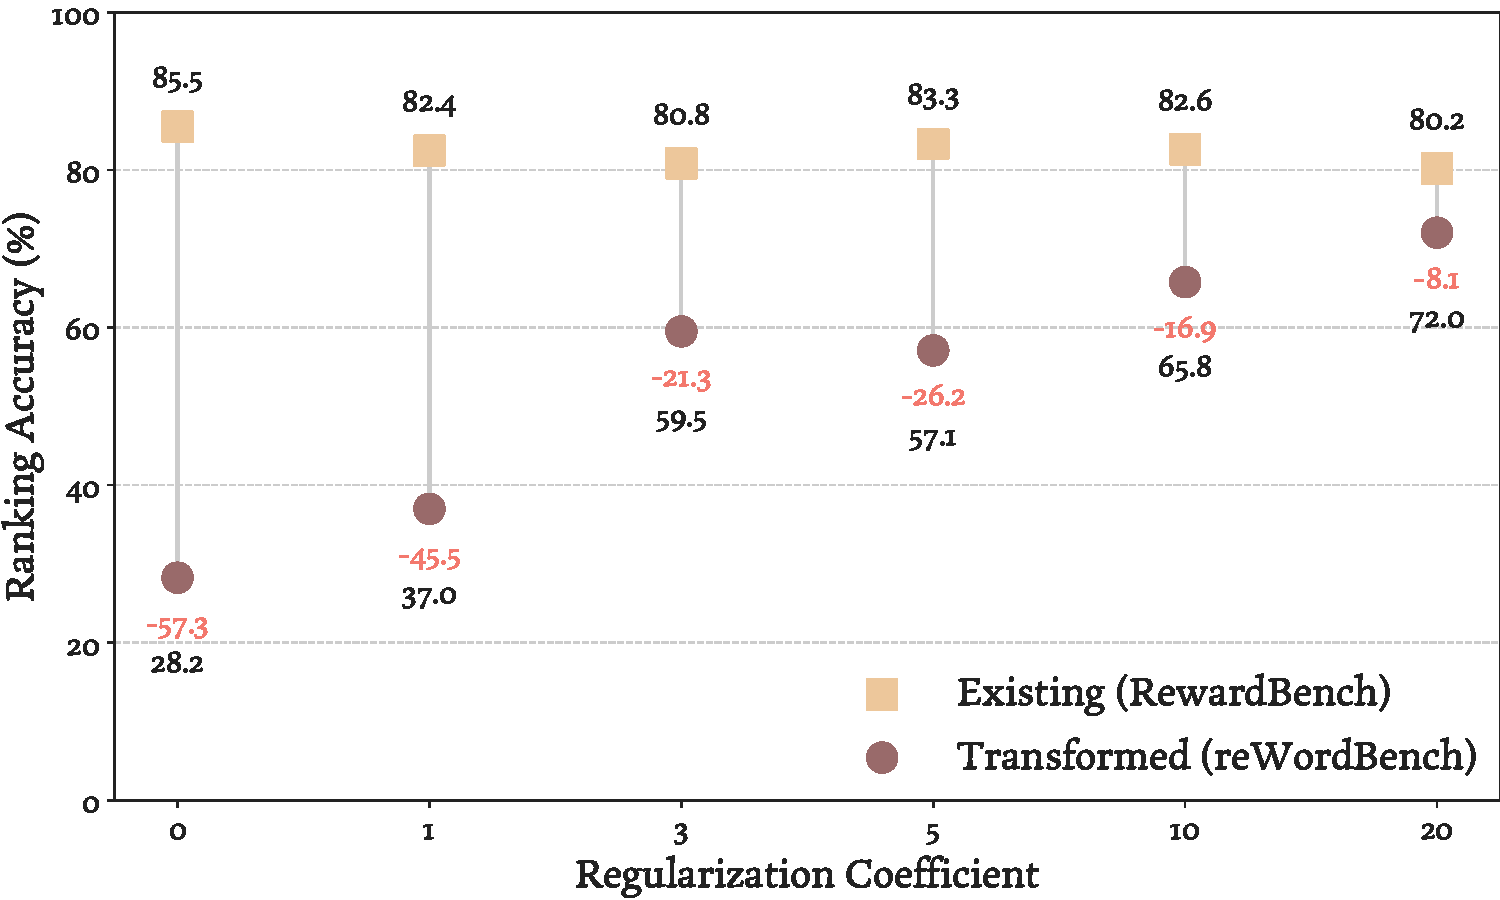
\includegraphics[width=0.5\columnwidth]{figures/consistency_rewardbench_ignore_chosen_above_quoted_coef.pdf}
    \else
    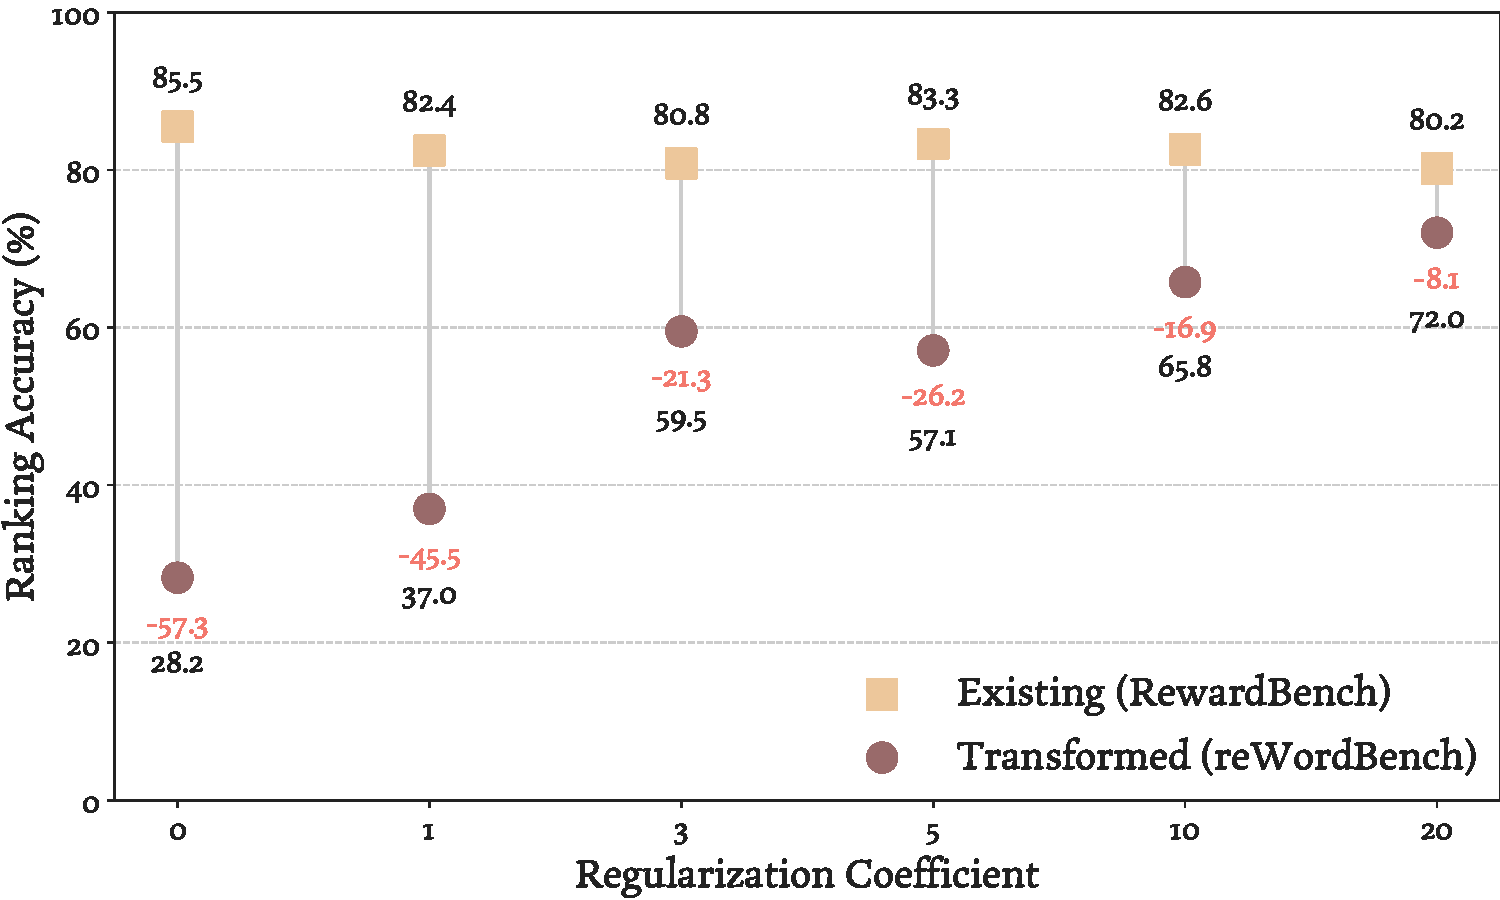
\includegraphics[width=0.9\columnwidth]{figures/consistency_rewardbench_ignore_chosen_above_quoted_coef.pdf}
    \fi
    \iflongversion
    \else
    \vspace{-2mm}
    \fi
    \caption{Ranking accuracy drop of our regularized reward models under the Ignore Above transformation (\S\ref{sec:controlled-transformations}), with different regularization strengths $\alpha$. The $x$-axis is not linear with respect to $\alpha$. \textbf{The RM robustness improves with increasing regularization strength.}}
    \iflongversion
    \else
    \vspace{-4mm}
    \fi
    \label{fig:robust-RM-coef}
\end{figure}

The robustness metric must also be complemented by a quality
\iflongversion
metric (because a perfectly robust but low-quality model would not be useful).
\else
metric.
\fi
We consider ranking accuracy on our \benchmark as a proxy for the RM quality in the wild as it suffers less from overfitting effects, unlike the potentially confounded original RewardBench accuracy (e.g., in the extreme, an entirely memorization-based approach could achieve 100\% original accuracy and 0\% transformed accuracy).
In the Chat, Chat Hard, and Reasoning subsets, our regularized RM achieves the highest ranking accuracy. This does not hold for the Safety subset, presumably because the HelpSteer2 data does not explicitly contain safety instances and so the model is not trained to be more robust on them.
Nonetheless, neither does HelpSteer2 explicitly contain coding and arithmetic data, and the improvement in the reasoning subset with our regularized RM is not \emph{a priori} expected.

\begin{figure*}[t!]
    \centering
    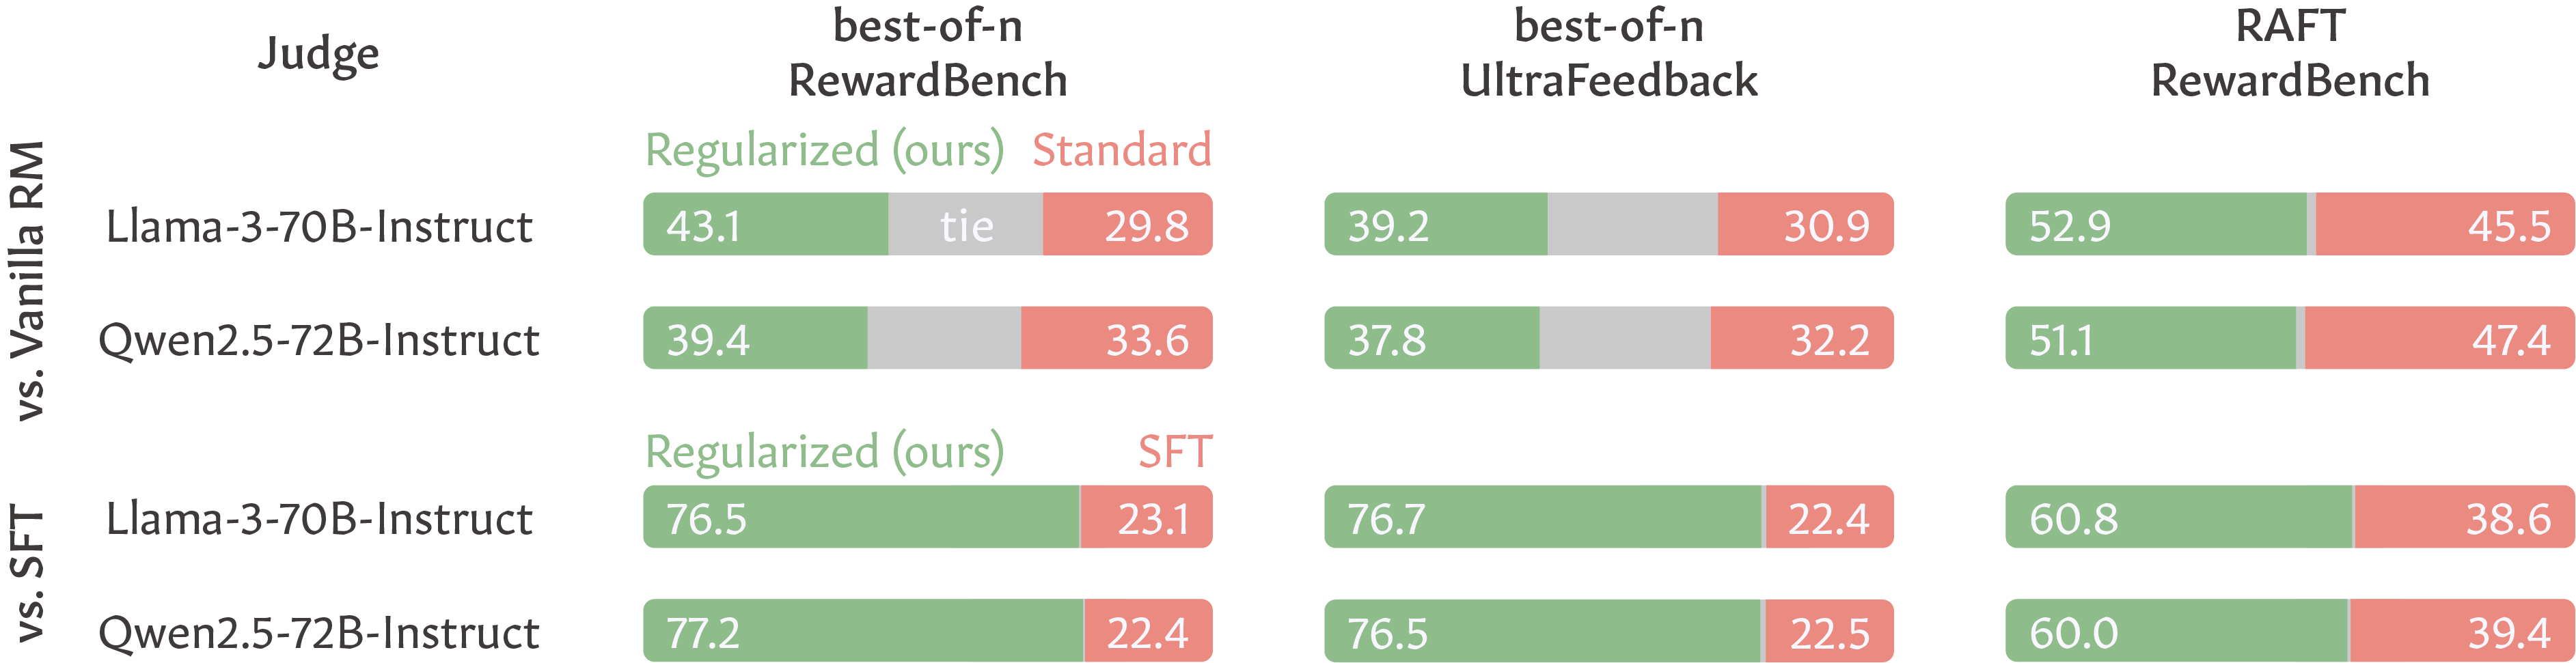
\includegraphics[width=\textwidth]{figures/winrate_cropped.png}
    \iflongversion
    \else
    \vspace{-2mm}
    \fi
    \caption{Comparing outputs aligned by our regularized RM vs. a standard-trained RM (and the \iflongversion unaligned \else\fi SFT model).
    We show how often (\%) each model wins according to an LM judge, or when they produce identical outputs (tie).
    \textbf{Our regularized RM consistently leads to better outputs in alignment compared to a standard-trained RM.}
    }
    \iflongversion
    \else
    \vspace{-2mm}
    \fi
    \label{fig:robust-RM-alignment-results}
\end{figure*}

We highlight that \textbf{regularization towards paraphrasing generalizes well to other diverse transformations in \benchmark} (Table~\ref{tab:robust-RM-rb-results}, last column), which is remarkable
\iflongversion
since many of our transformations are distinct from the paraphrase-based training instances.
\else
since many of our transformations are distinct from the paraphrase-based training instances.
\fi
Similarly, Figure~\ref{fig:robust-RM-coef} shows the effect of regularization strength for the Ignore Above transformation.
\iflongversion
Increasing the regularization coefficient $\alpha$
\else
Increasing regularization
\fi
leads to better model robustness, again even though it is of a very different nature to paraphrasing.\footnote{The optimal $\alpha$ that balances accuracy and robustness differs depending on the specific transformation; overall, we use $\alpha=10$, as mentioned in \S\ref{sec:exp-setup}.}
This further corroborates the effectiveness of our method.

\subsection{Robust RM in Downstream Alignment} \label{sec:robust-rm-in-alignment}

We consider two alignment methods that require an RM. The first is \bon, an inference-time algorithm, where we sample $n=64$ responses from the SFT model and use the highest RM-scored one as the output. This is an empirically strong method that outperforms alternatives that require training~\citepia{gao2022scaling,rafailov2023direct,MudgalLGLWHCCCS24}.
We use the prompts from either RewardBench (2985 instances) or UltraFeedback~(\citealp{cui2024ultrafeedbackboostinglanguagemodels}; only the first 3,000 due to its size).
Additional training details are in \S\ref{sec:training-details}.

We also consider a training-based alignment method where we finetune the SFT model using \bon-chosen
\iflongversion
responses~\citep{singh2024beyond,dong2023raft,yasunaga2024almaalignmentminimalannotation}.\footnote{Past work has suggested performing this procedure iteratively~\citep{dong2023raft}, though we did not observe substantial quality gain from doing so in our setting.}
\else
responses~\citep{singh2024beyond,dong2023raft,yasunaga2024almaalignmentminimalannotation}.
\fi
Specifically, we compute \bon on all UltraFeedback prompts
(discarding the original responses)
and use the RM-chosen response to finetune the SFT model. During inference, we sample from the SFT model once. Again, we use $n=64$.
We call this method ``RAFT''~\citep{dong2023raft}.\footnote{We chose this method due to its simplicity and effectiveness found in prior work. We expect qualitatively similar results for alternative methods and leave them to future work.
}

We auto-evaluate the alignment outputs using
SOTA LM judges.
We present the prompt and two responses generated by two systems, ask the LM judge which one is preferred, and compute the win rate.
This is a standard protocol that has been verified to correlate well with human judgments for dialogs~\citepia{lee2023rlaif,rafailov2023direct,an-etal-2024-l,mu2023learning}.
To further ensure the robustness of results, we consider two different LM judges, Llama-3-70B-Instruct and Qwen2.5-72B-Instruct~\citep{qwen2.5}, which have undergone distinct pretraining and post-training stages.
In \S\ref{sec:length-effect}, we also verify that more strictly controlling for length, a common bias of LM
\iflongversion
judges~\citep{wang2023how,singhal2023long},
\else
judges~\citep{singhal2023long},
\fi
does not qualitatively affect our results.

From Figure~\ref{fig:robust-RM-alignment-results} (top), across all alignment settings, we see a consistent improvement of our regularized RM over a conventionally trained standard RM.
This means that the robustness of our regularized RM extends to downstream alignment where it leads to higher-quality outputs.
This also manifests similarly when judged by different evaluator LMs, demonstrating its robustness.
Figure~\ref{fig:robust-RM-alignment-results} (bottom) shows that our aligned models are decent, with 60\%--80\% win rates against the SFT model.
